\chapter{Remarks about our study}
In this chapter we are going to describe in detail the specifications of the simulations we are going to work with, as well as the method for determining the halo shapes. This shapter is mainly to thoroughly explain how are we going to do everything that we are going to do.\\

\section{The Auriga simulations}
State all the important specs of the Auriga simulations. On the first paragraph.\\

Talk about the different degrees of realism in this simulation> DM, MHD, resolution levels. State the importance of these aspects for the soundness (look better word) of the studies.\\

\begin{figure}[!ht]
    \centering
    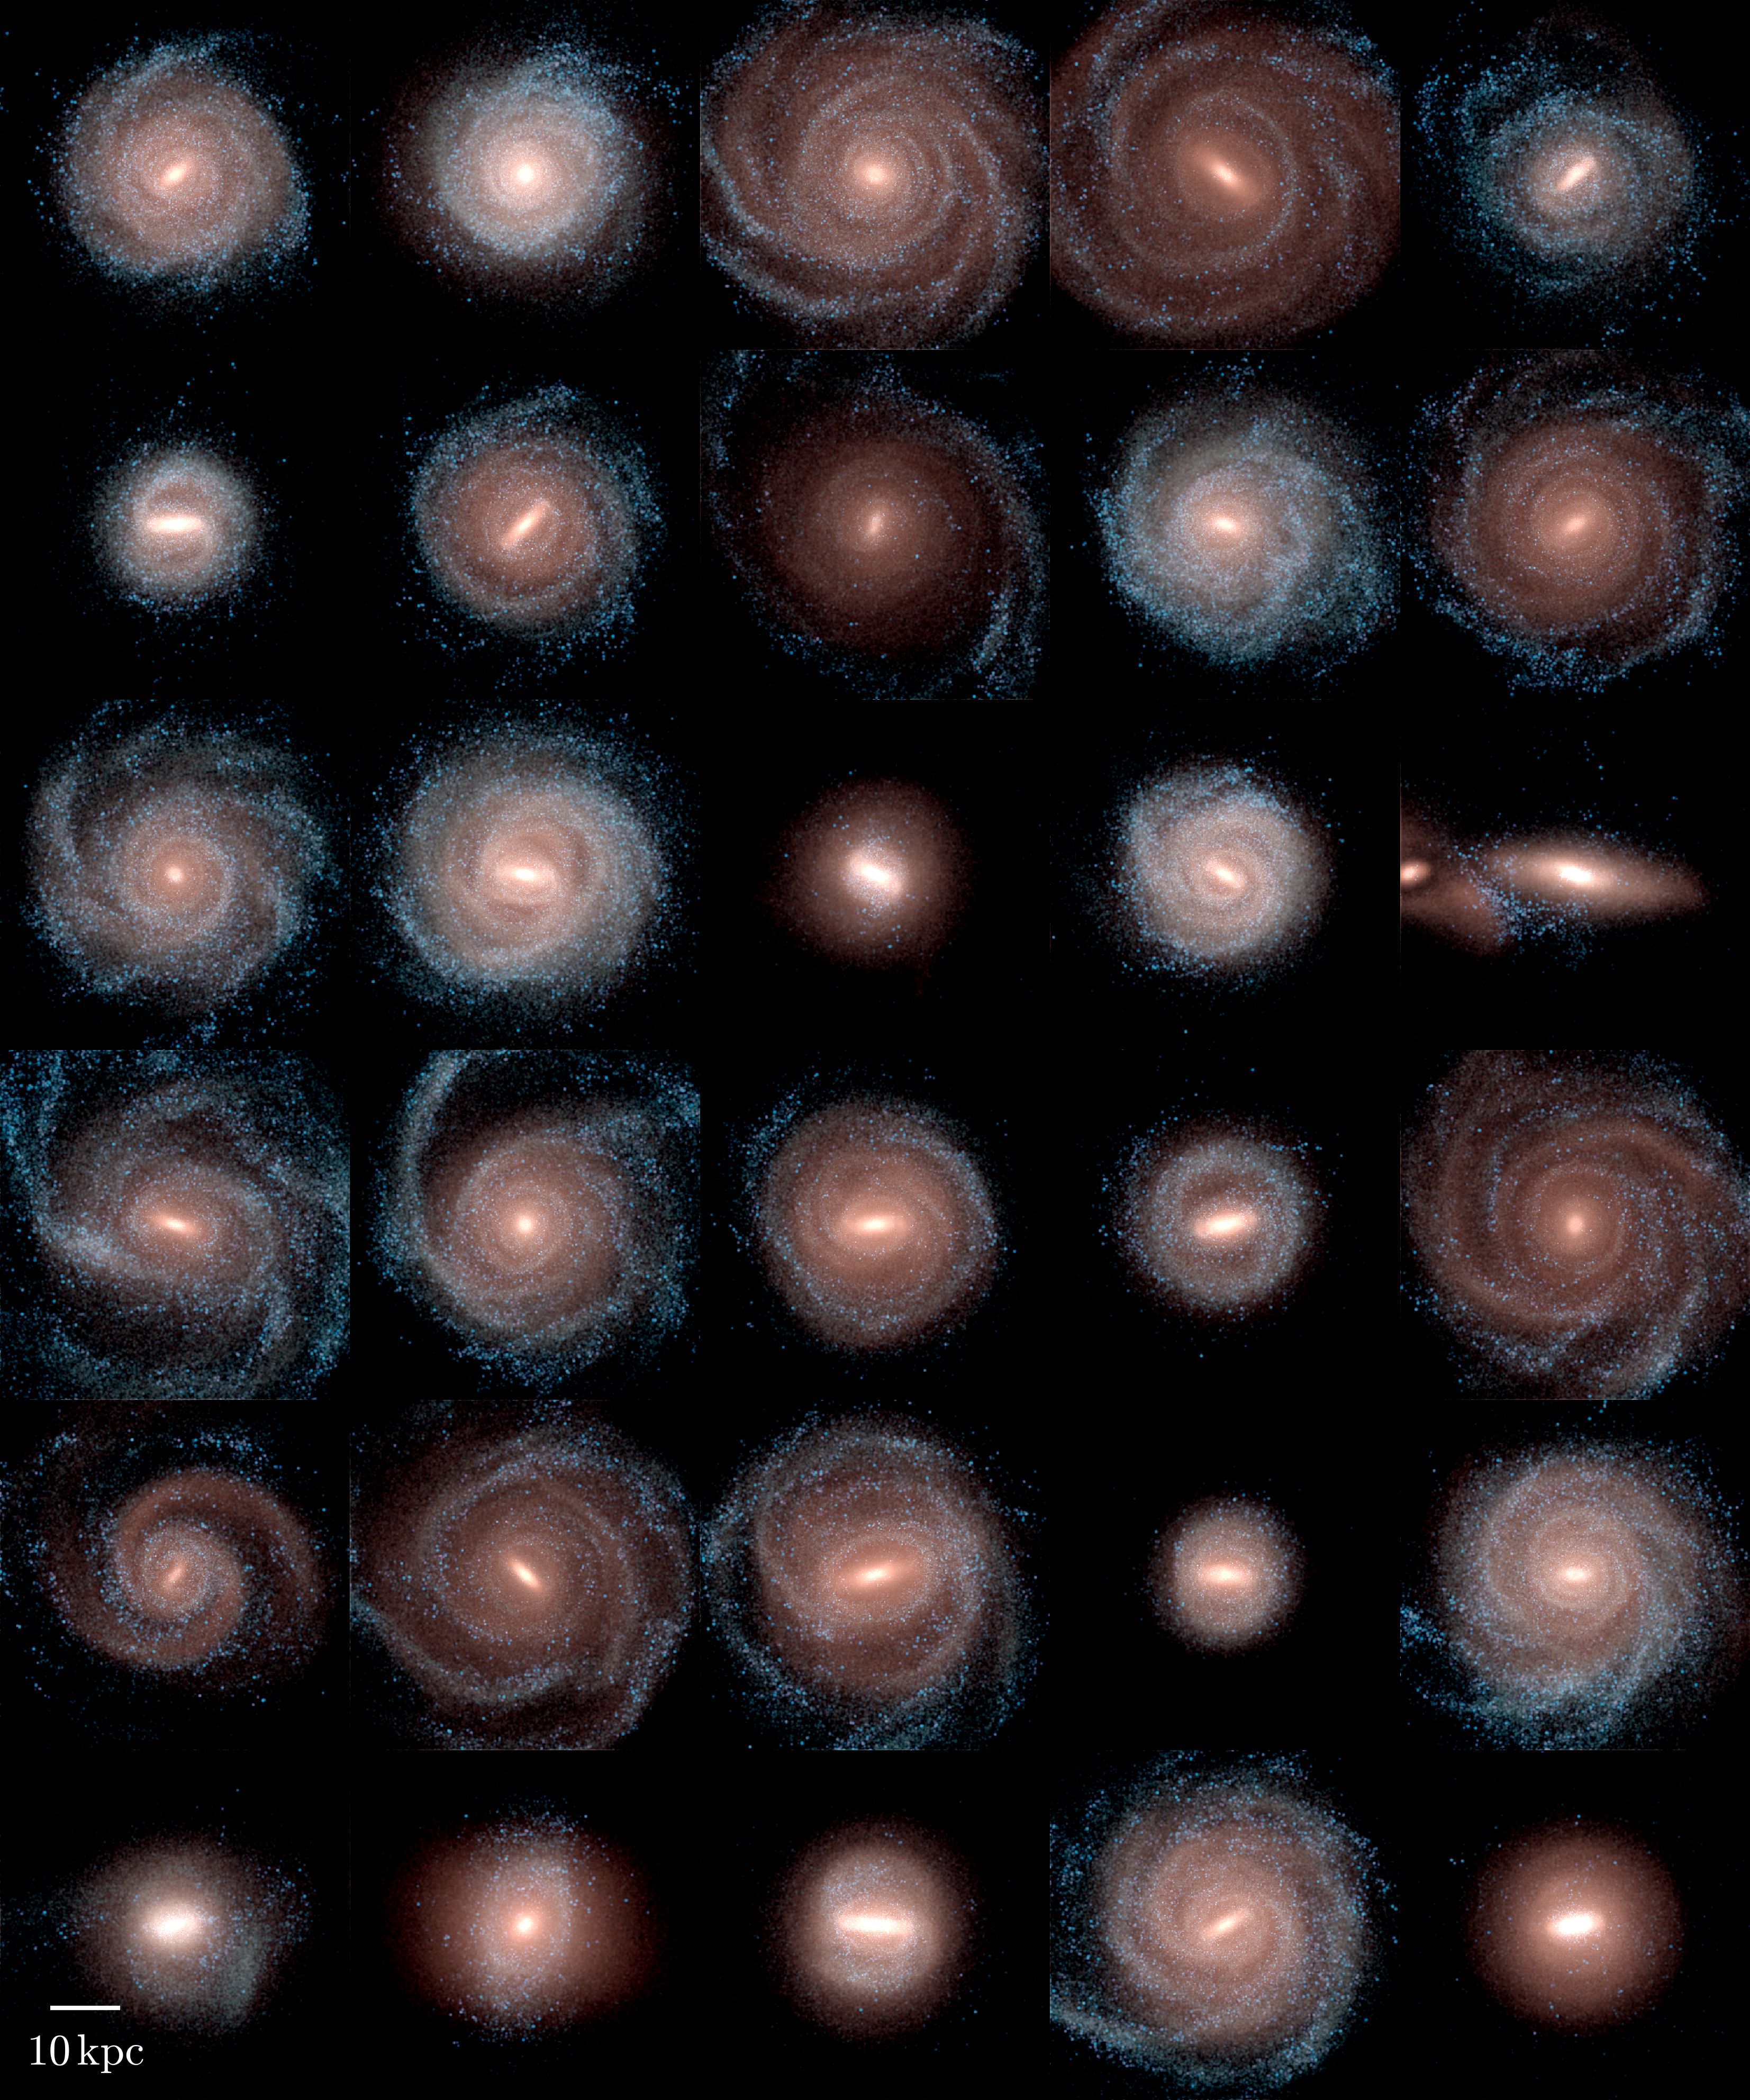
\includegraphics[width=0.8\textwidth]{./pics/Auriga.png}
    \caption{Set of 30 MW-like simulations, taken from http://auriga.h-its.org/}
    \label{fig:auriga}
\end{figure}

\section{Determining the halo shape}
Start saying that there is no unique method for determining the shape at a specific radius. In general this process is not trivial and there are many different(in theory) approaches which produce esentially the same results \cite{Vera-Ciro2010}. Mention that we are going to use method by Allgood et al 2006 \cite{AllGood2006} following the steps by Vera-Ciro2010.\\

The method starts with particles enclosed within a sphere, we calculate the reduced inertia tensor:

\begin{equation}
I_{ij} = \sum_k \frac{x_k^{(i)}x_k^{(j)}}{d^2_k},
\label{eq:inertia}
\end{equation}

that is not sufficient, which is why we recalculate until we achieve convergence. Present this recalculation explicitly with a scale transformation which intuitively means that our ellipse is becoming a sphere under that transformation which at the end is fully consistent (find better words).

\begin{align}
(x,y,z) &\rightarrow (x,y/q,z/s) \label{eq:scale}\\
q &=  b/a \nonumber \\
s &= c/a \nonumber ,
\end{align}

Specify that with this process we obtain both the radial profile and the historical shape by simply applying this method at different radii and redshifts.
